\chapter{Dynamic Model \label{ch:model}}


\section{Non-linear Model}

This section describes the dynamic modeling used to perform the quadrotor control, based on the study carried out in \cite{modelamiento, modelamientoPDAFC, modelamientoNCQ}. This model represents the quadrotor as a solid symmetrical object subject to a total thrust and three torques, without considering the dynamics of the actuators.
\begin{figure*}
\begin{center}
% Use the relevant command to insert your figure file.
% For example, with the graphicx package use
  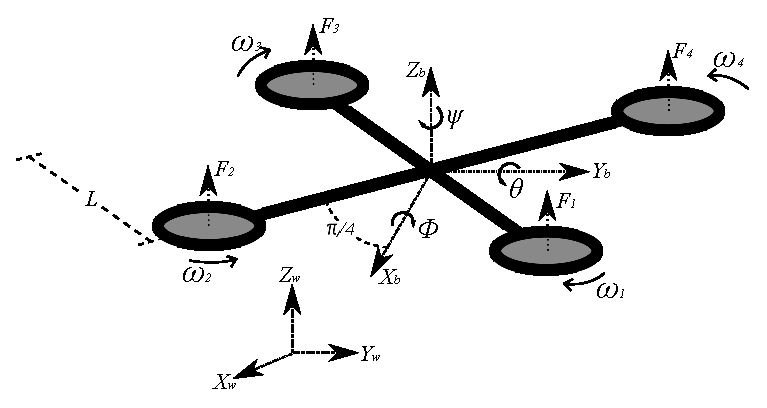
\includegraphics[width=0.9\textwidth]{quadcopter1.eps}
% figure caption is below the figure
\caption{Quadrotor squeme with movement axis and thrust forces.} 
    \label{fig:marcoreferencia}
    \end{center}
\end{figure*}
\\\\The general coordinates representing the position and attitude of the quadrotor are defined as
\begin{equation}
	q=\begin{bmatrix}
	\xi & \eta
	\end{bmatrix}^{T},
	\label{ec:coorgenerales}
\end{equation}
where $\xi=\begin{bmatrix}
x & y & z
\end{bmatrix}^{T}$ is the vector representing the position of the center of mass of the quadrotor relative to the body reference frame shown in Fig. \ref{fig:marcoreferencia} and $\eta=\begin{bmatrix}
\psi & \theta & \phi
\end{bmatrix}^{T}$ represent the quadrotor's attitude.
\\\\
The Lagrangian of the quadrotor is defined by
\begin{equation}
	L(q,\dot{q})=K_{trans}+K_{rot} - U,	
	\label{ec:lagrangiano}
\end{equation}
where $ K_{trans} = \dfrac{m}{2}\dot{\xi}^{T}\dot{\xi} $ is the translational kinetic energy, $ K_{rot} = \dfrac{1}{2}\dot{\eta}^{T}J\dot{\eta} $ is the rotational kinetic energy, $ U=mgz $ is the potential energy, $m$ is the quadrotor's mass , $z$ is the quadrotor's elevation, $g$ is the gravity acceleration magnitude, and $J$ is the inertial matrix. The dynamic model of the quadrotor is derived from the Euler-Lagrange equation
\begin{equation}
	\dfrac{d}{dt}\dfrac{\partial L}{\partial \dot{q}}-\dfrac{\partial L}{\partial q}=
	\begin{bmatrix}
	F_{\xi}\\
	\tau
	\end{bmatrix},
	\label{ec:eulerlag}
 \end{equation} 
where $F_{\xi}=R_{b}^{w}\hat{F_{b}}$ is the translational force applied to the quadrotor by the four motors, $\tau$ contains the rolling, pitching and yawing torques, and 
\begin{equation}
R_{b}^{w} = \begin{bmatrix}
c\theta c\psi & c\psi s\theta s\phi-c\phi s\psi & s\phi s\psi+c\phi c\psi s\theta\\
c\theta s\psi & s\psi s\theta s\phi+c\phi c\psi & c\phi s\psi s\theta - s\phi c\psi\\
-s\theta & c\theta s\phi & c\theta c\phi
\end{bmatrix}
\end{equation}
is the rotation matrix from the body to the Earth frame where $c\theta = \cos\theta$ and $s\theta = \sin\theta$.
\\\\
In the quadrotor's body frame, the translational force $\hat{F_{b}}$ is only applied in the $z_{b}$ axis as shown in Fig. \ref{fig:marcoreferencia}. This force is represented by
\begin{equation}
	\hat{F_{b}}=\begin{pmatrix}
	0\\
	0\\
	u
	\end{pmatrix} = \begin{pmatrix}
	0\\
	0\\
	\sum_{i=1}^{4}F_{i}
	\end{pmatrix}  ,
 \label{ec:fuerzas}
 \end{equation} 
with $ F_{i} $ being the force, in N, exerted by the motor $ M_{i}$, as shown in Fig. \ref{fig:marcoreferencia}.
\\\\
The force $ F_{i} $ has a linear dependency with the square of the motor angular velocity, defined as
\begin{equation}
	F_{i}=k_{i}w_{i}^{2},
	\label{ec:fi}
\end{equation}
where $ w_{i} $ is the angular velocity of the motor, and $ k_{i} $ is a proportional constant. However, in practice $F_{i}$ must be set using the PWM signal input of an ESC. The thrust-PWM relation is found experimentally and is shown in Section \ref{sec:Implementation}.
\\\\
The rolling, pitching and yawing torques contained in vector $\tau$, are generated using the force exerted by each motor as
\begin{equation}
	\tau = \begin{bmatrix}
	\tau_{\psi}\\
	\tau_{\theta}\\
	\tau_{\phi}
	\end{bmatrix} = \begin{bmatrix}
								T_{1} + T_{3} - T_{2} - T_{4}\\
								Lcos(\pi/4)(F_{3}+F_{4}-F_{2}-F_{1})\\
								Lcos(\pi/4)(F_{2}+F_{3}-F_{1}-F_{4})
							\end{bmatrix},
	\label{ec:torques}						
\end{equation}
where $ T_{i} $ is the torque produced by each motor along the $z_{b}$ axis, $ L $ is the distance between each motor's rotor and the quadrotor's center of mass, and $Lcos(\pi/4)$ is the real distance between the point of application of the rolling and pitching torques and the quadrotor's center of mass along the $x_b$ and $y_b$ axes \cite{Faessler2016}.\\\\
The Euler-Lagrange equations can be divided in two parts, one for the $\xi$ coordinates and another for the $\eta$ coordinates, getting
\begin{equation}
\label{eqn:E-L1}
\ddot{\xi} =
\begin{bmatrix}
\ddot{x} \\ \ddot{y} \\ \ddot{z}
\end{bmatrix} 
=
\begin{bmatrix}
\frac{u_{1}}{m}(\cos\phi\sin\theta\cos\psi + \sin\phi\sin\psi) \\
 \frac{u_{1}}{m}(\cos\phi\sin\theta\sin\psi - \sin\phi\cos\psi) \\
\frac{u_{1}}{m}(\cos\phi\cos\theta) - g
\end{bmatrix},
\end{equation}
\begin{equation}
\label{eqn:E-L2}
\ddot{\eta} =
\begin{bmatrix}
\ddot{\psi} \\ \ddot{\theta} \\ \ddot{\phi}
\end{bmatrix} 
 =
\begin{bmatrix}
\dot{\phi}\dot{\theta}\dfrac{J_{xx}-J_{yy}}{J_{zz}} + \dfrac{u_{2}}{J_{zz}} \\
\dot{\phi}\dot{\psi}\dfrac{J_{zz}-J_{xx}}{J_{yy}} + \dfrac{u_{3}}{J_{yy}} \\
 \dot{\theta}\dot{\psi}\dfrac{J_{yy}-J_{zz}}{J_{xx}} +  \dfrac{u_{4}}{J_{xx}}
\end{bmatrix},
\end{equation}
where, $\begin{bmatrix}
u_{1},\ u_{2},\ u_{3}, \ u_{4}
\end{bmatrix}^{T} = \begin{bmatrix}
u,\ \tau_{\psi},\ \tau_{\theta},\ \tau_{\phi}
\end{bmatrix}^{T} $, and $ (J_{xx}, J_{yy}, J_{zz}) $ are the moments of inertia around the quadrotor's body axes \cite{Emam2016, Badr2016}.
\\\\
The Euler-Lagrange equations in (\ref{eqn:E-L1}) and (\ref{eqn:E-L2}) are linearized using their Jacobian around the hover state where $\begin{bmatrix}
\eta,\ \dot{\eta},\ \dot{\xi}
\end{bmatrix} \to \begin{bmatrix}
0,\ 0,\ 0
\end{bmatrix}$, getting
\begin{equation}
\label{eqn:linear}
\ddot{q}
=
\begin{bmatrix}
g\theta \\
g\phi\\
u_{1}/m \\
u_{2}/J_{zz} \\
u_{3}/J_{yy} \\
u_{4}/J_{xx}
\end{bmatrix},
\end{equation}
that is a simplified representation of the quadrotor complete model found in \cite{Bouabdallah2007}.



\section{Linearized Model}
\setcounter{MaxMatrixCols}{20}

The linearised model of the quad-rotor helicopter written as a state space model is given by

\begin{align*}
\dot{x}(t)= & Ax(t)+Bu(t),\\
r(t)= & Cx(t),
\end{align*}
where
\begin{align*}
A  = & 
\begin{bmatrix}
0 & 1 & 0 & 0 & 0 & 0 & 0 & 0 & 0 & 0 & 0 & 0\\
0 & 0 & 0 & 0 & 0 & 0 & 0 & 0 & -g & 0 & 0 & 0\\
0 & 0 & 0 & 1 & 0 & 0 & 0 & 0 & 0 & 0 & 0 & 0\\
0 & 0 & 0 & 0 & 0 & 0 & 0 & 0 & 0 & 0 & g & 0\\
0 & 0 & 0 & 0 & 0 & 1 & 0 & 0 & 0 & 0 & 0 & 0\\
0 & 0 & 0 & 0 & 0 & 0 & 0 & 0 & 0 & 0 & 0 & 0\\
0 & 0 & 0 & 0 & 0 & 0 & 0 & 1 & 0 & 0 & 0 & 0\\
0 & 0 & 0 & 0 & 0 & 0 & 0 & 0 & 0 & 0 & 0 & 0\\
0 & 0 & 0 & 0 & 0 & 0 & 0 & 0 & 0 & 1 & 0 & 0\\
0 & 0 & 0 & 0 & 0 & 0 & 0 & 0 & 0 & 0 & 0 & 0\\
0 & 0 & 0 & 0 & 0 & 0 & 0 & 0 & 0 & 0 & 0 & 1\\
0 & 0 & 0 & 0 & 0 & 0 & 0 & 0 & 0 & 0 & 0 & 0
\end{bmatrix}
\end{align*}
\begin{align*}
B = & 
\begin{bmatrix}
0 & 0 & 0 & 0 & 0 & \frac{1}{m} & 0 & 0 & 0 & 0 & 0 & 0\\
0 & 0 & 0 & 0 & 0 & 0 & 0 & 1 & 0 & 0 & 0 & 0\\
0 & 0 & 0 & 0 & 0 & 0 & 0 & 0 & 0 & 1 & 0 & 0\\
0 & 0 & 0 & 0 & 0 & 0 & 0 & 0 & 0 & 0 & 0 & 1
\end{bmatrix}^T
\end{align*}
%
\begin{align*}
C  = & 
\begin{bmatrix}
1 & 0 & 0 & 0 & 0 & 0 & 0 & 0 & 0 & 0 & 0 & 0\\
0 & 0 & 1 & 0 & 0 & 0 & 0 & 0 & 0 & 0 & 0 & 0\\
0 & 0 & 0 & 0 & 1 & 0 & 0 & 0 & 0 & 0 & 0 & 0
\end{bmatrix}^T
\end{align*}

with the parameters  

$m=0.64 $ kg, 

$g=9.81$ m/s.


The state vector is defined as

\begin{align*}
x(t)=&
\begin{bmatrix}
r_x & \dot{r}_x & r_y & \dot{r}_y & r &\dot{r}_z 
\end{bmatrix}^T,
\end{align*}
and the control inputs as
\begin{align*}
u(t)=&
\begin{bmatrix}
u_1 & u_2 &u_3 & u_4
\end{bmatrix}^T,
\end{align*}

and the output vector is defined as

\begin{align*}
r(t)=
\begin{bmatrix}
r_{x} & r_{y} & r_{z}
\end{bmatrix}^T.
\end{align*}
